\documentclass[11pt,a4paper]{article}
\usepackage[margin=2.5cm]{geometry}
\usepackage{graphicx}
\usepackage{booktabs}
\usepackage{xcolor}
\usepackage{hyperref}
\usepackage{amsmath}
\usepackage{float}
\usepackage{caption}
\usepackage{subcaption}
\usepackage{enumitem}
\usepackage{fancyhdr}

\definecolor{akblue}{HTML}{1f77b4}
\definecolor{bcgreen}{HTML}{2ca02c}
\definecolor{ssorange}{HTML}{ff7f0e}
\definecolor{jdfred}{HTML}{d62728}
\definecolor{orpurple}{HTML}{9467bd}
\definecolor{canpink}{HTML}{e377c2}
\definecolor{alertred}{HTML}{cc0000}
\definecolor{okgreen}{HTML}{228B22}

\pagestyle{fancy}
\fancyhf{}
\rhead{SSWD Calibration}
\lhead{W75--W84 Report}
\rfoot{Page \thepage}

\title{\textbf{Calibration Report: $K_{1/2}$ / $P_{\text{env,max}}$ Sweep}\\[0.3em]
\large Runs W75--W84 with Dynamic $P_{\text{env}}$}
\author{SSWD EvoEpi Model Calibration}
\date{March 4, 2025}

\begin{document}
\maketitle
\thispagestyle{fancy}

% ═══════════════════════════════════════════════════════════════
\section{Executive Summary}
% ═══════════════════════════════════════════════════════════════

W75--W84 tested lifting recovery levels from W71 (the previous best run with dynamic $P_{\text{env}}$), which had the correct north--south gradient shape but all recovery values 3--5$\times$ too suppressed. The sweep varied $K_{1/2}$ (600K, 800K, 1M) and $P_{\text{env,max}}$ (1000, 1500, 2000) to find the right overall recovery level while maintaining the latitudinal gradient.

\subsection*{Key Findings}

\begin{enumerate}[leftmargin=*]
    \item \textbf{\textcolor{alertred}{$P_{\text{env,max}}$ has ZERO effect.}} Runs with the same $K_{1/2}$ but different $P_{\text{env,max}}$ produce \emph{identical} results to every decimal place. W75$=$W78$=$W81, W76$=$W79$=$W82, W77$=$W80. Dynamic $P_{\text{env}}$ completely dominates; the static cap is never reached.

    \item \textbf{$K_{1/2}$ controls overall recovery level uniformly.} Increasing $K_{1/2}$ lifts \emph{all} regions proportionally---it acts as a global multiplier, not a gradient shaper. No differential north--south effect.

    \item \textbf{Gradient collapsed.} W71 achieved a 35$\times$ gradient (AK-PWS/CA-N ratio). At $K_{1/2}$=800K (W76), while AK-PWS hits 57.1\% (target: 50\%) and AK-FS hits 21.2\% (target: 20\%), the gradient collapsed to just 1.6$\times$---southern regions recover nearly as much as Alaska.

    \item \textbf{Floor parameter ($P_{\text{env,floor}}$) is too weak.} Reducing floor from 100 to 75 (W83 vs W76) produced only marginal improvement. The floor (minimum disease pressure) is insufficient to suppress southern recovery at high $K_{1/2}$.

    \item \textbf{Best overall RMSE is W71} (0.692), despite all values being too low. The W75--W84 sweep worsened RMSE (1.16--1.44) because lifting the north correctly also massively overshoot the south.
\end{enumerate}

\subsection*{Implication}
A single global parameter ($K_{1/2}$) cannot simultaneously produce correct AK recovery \emph{and} correct southern suppression. The model needs a mechanism that differentially suppresses recovery in the south---either latitude-dependent $K_{1/2}$, stronger floor effects, or an entirely different disease pressure gradient.


% ═══════════════════════════════════════════════════════════════
\section{Methods}
% ═══════════════════════════════════════════════════════════════

\subsection{Parameter Sweep Design}

All runs share the following fixed parameters:
\begin{itemize}[nosep]
    \item Dynamic $P_{\text{env}}$: enabled ($\alpha_{\text{env}}=0.1$)
    \item $\delta_{\text{env}} = 0.02$
    \item Cumulative dose threshold: 1000
    \item Wavefront $D_P = 300$, max range = 3000
    \item Settler survival: 0.002
    \item $K = 5000$, 13 years (2012--2024), seed = 42
\end{itemize}

The sweep varied three parameters:

\begin{table}[H]
\centering
\caption{Parameter sweep design for W75--W84}
\label{tab:params}
\begin{tabular}{lccc}
\toprule
\textbf{Run} & \textbf{$K_{1/2}$} & \textbf{$P_{\text{env,max}}$} & \textbf{$P_{\text{env,floor}}$} \\
\midrule
W71 (ref) & 400K & 2000 & 100 \\
\midrule
W75 & 600K & 2000 & 100 \\
W76 & 800K & 2000 & 100 \\
W77 & 1,000K & 2000 & 100 \\
W78 & 600K & 1500 & 100 \\
W79 & 800K & 1500 & 100 \\
W80 & 1,000K & 1500 & 100 \\
W81 & 600K & 1000 & 100 \\
W82 & 800K & 1000 & 100 \\
W83 & 800K & 2000 & 75 \\
W84 & 800K & 1500 & 75 \\
\bottomrule
\end{tabular}
\end{table}

\subsection{Recovery Metric}
Recovery fraction = final population / pre-crash peak (maximum of first 3 years). RMSE is computed on log-scale errors across 8 target regions.

\subsection{Calibration Targets}

\begin{table}[H]
\centering
\caption{Target recovery fractions by region}
\begin{tabular}{lcccccccc}
\toprule
& AK-PWS & AK-FN & AK-FS & BC-N & SS-S & JDF & OR & CA-N \\
\midrule
Target (\%) & 50 & 50 & 20 & 20 & 5 & 2 & 0.25 & 0.1 \\
\bottomrule
\end{tabular}
\end{table}


% ═══════════════════════════════════════════════════════════════
\section{Results}
% ═══════════════════════════════════════════════════════════════

\subsection{Summary Table}

\begin{table}[H]
\centering
\caption{Recovery percentages and RMSE for all runs. \textcolor{okgreen}{Green} = within 2$\times$ of target. Values that match exactly across runs confirm $P_{\text{env,max}}$ irrelevance.}
\label{tab:results}
\small
\begin{tabular}{lccr|rrrrrrrr|c}
\toprule
\textbf{Run} & $K_{1/2}$ & $P_{\text{max}}$ & \textbf{floor} & \textbf{PWS} & \textbf{FN} & \textbf{FS} & \textbf{BC-N} & \textbf{SS-S} & \textbf{JDF} & \textbf{OR} & \textbf{CA-N} & \textbf{RMSE} \\
\midrule
Target & --- & --- & --- & 50.0 & 50.0 & 20.0 & 20.0 & 5.0 & 2.0 & 0.25 & 0.10 & --- \\
\midrule
W71 & 400K & 2000 & 100 & 10.5 & 3.3 & 3.7 & 7.0 & 1.6 & 7.1 & 1.3 & 0.3 & \textbf{0.692} \\
\midrule
W75 & 600K & 2000 & 100 & 27.5 & 16.7 & 13.2 & 15.9 & 24.5 & 39.7 & 12.5 & 20.4 & 1.158 \\
W78 & 600K & 1500 & 100 & 27.5 & 16.7 & 13.2 & 15.9 & 24.5 & 39.7 & 12.5 & 20.4 & 1.158 \\
W81 & 600K & 1000 & 100 & 27.5 & 16.7 & 13.2 & 15.9 & 24.5 & 39.7 & 12.5 & 20.4 & 1.158 \\
\midrule
W76 & 800K & 2000 & 100 & \textcolor{okgreen}{57.1} & 34.0 & \textcolor{okgreen}{21.2} & 37.3 & 44.1 & 43.4 & 36.8 & 34.9 & 1.321 \\
W79 & 800K & 1500 & 100 & \textcolor{okgreen}{57.1} & 34.0 & \textcolor{okgreen}{21.2} & 37.3 & 44.1 & 43.4 & 36.8 & 34.9 & 1.321 \\
W82 & 800K & 1000 & 100 & \textcolor{okgreen}{57.1} & 34.0 & \textcolor{okgreen}{21.2} & 37.3 & 44.1 & 43.4 & 36.8 & 34.9 & 1.321 \\
\midrule
W77 & 1M & 2000 & 100 & 74.2 & \textcolor{okgreen}{58.1} & 53.0 & 55.7 & 61.1 & 61.3 & 51.9 & 55.2 & 1.444 \\
W80 & 1M & 1500 & 100 & 74.2 & \textcolor{okgreen}{58.1} & 53.0 & 55.7 & 61.1 & 61.3 & 51.9 & 55.2 & 1.444 \\
\midrule
W83 & 800K & 2000 & 75 & \textcolor{okgreen}{60.0} & 40.1 & 27.8 & 36.6 & 32.0 & 33.6 & 31.7 & 38.8 & 1.293 \\
W84 & 800K & 1500 & 75 & \textcolor{okgreen}{60.0} & 40.1 & 27.8 & 36.6 & 32.0 & 33.6 & 31.7 & 38.8 & 1.293 \\
\bottomrule
\end{tabular}
\end{table}

\textbf{Note:} W83$=$W84 confirms $P_{\text{env,max}}$ independence extends to floor=75 runs as well. Effectively, the entire sweep has only \textbf{4 distinct outcomes}: $K_{1/2}$=600K, 800K, 1M with floor=100, and $K_{1/2}$=800K with floor=75.

\subsection{Key Runs: Recovery Time Series}

\begin{figure}[H]
\centering
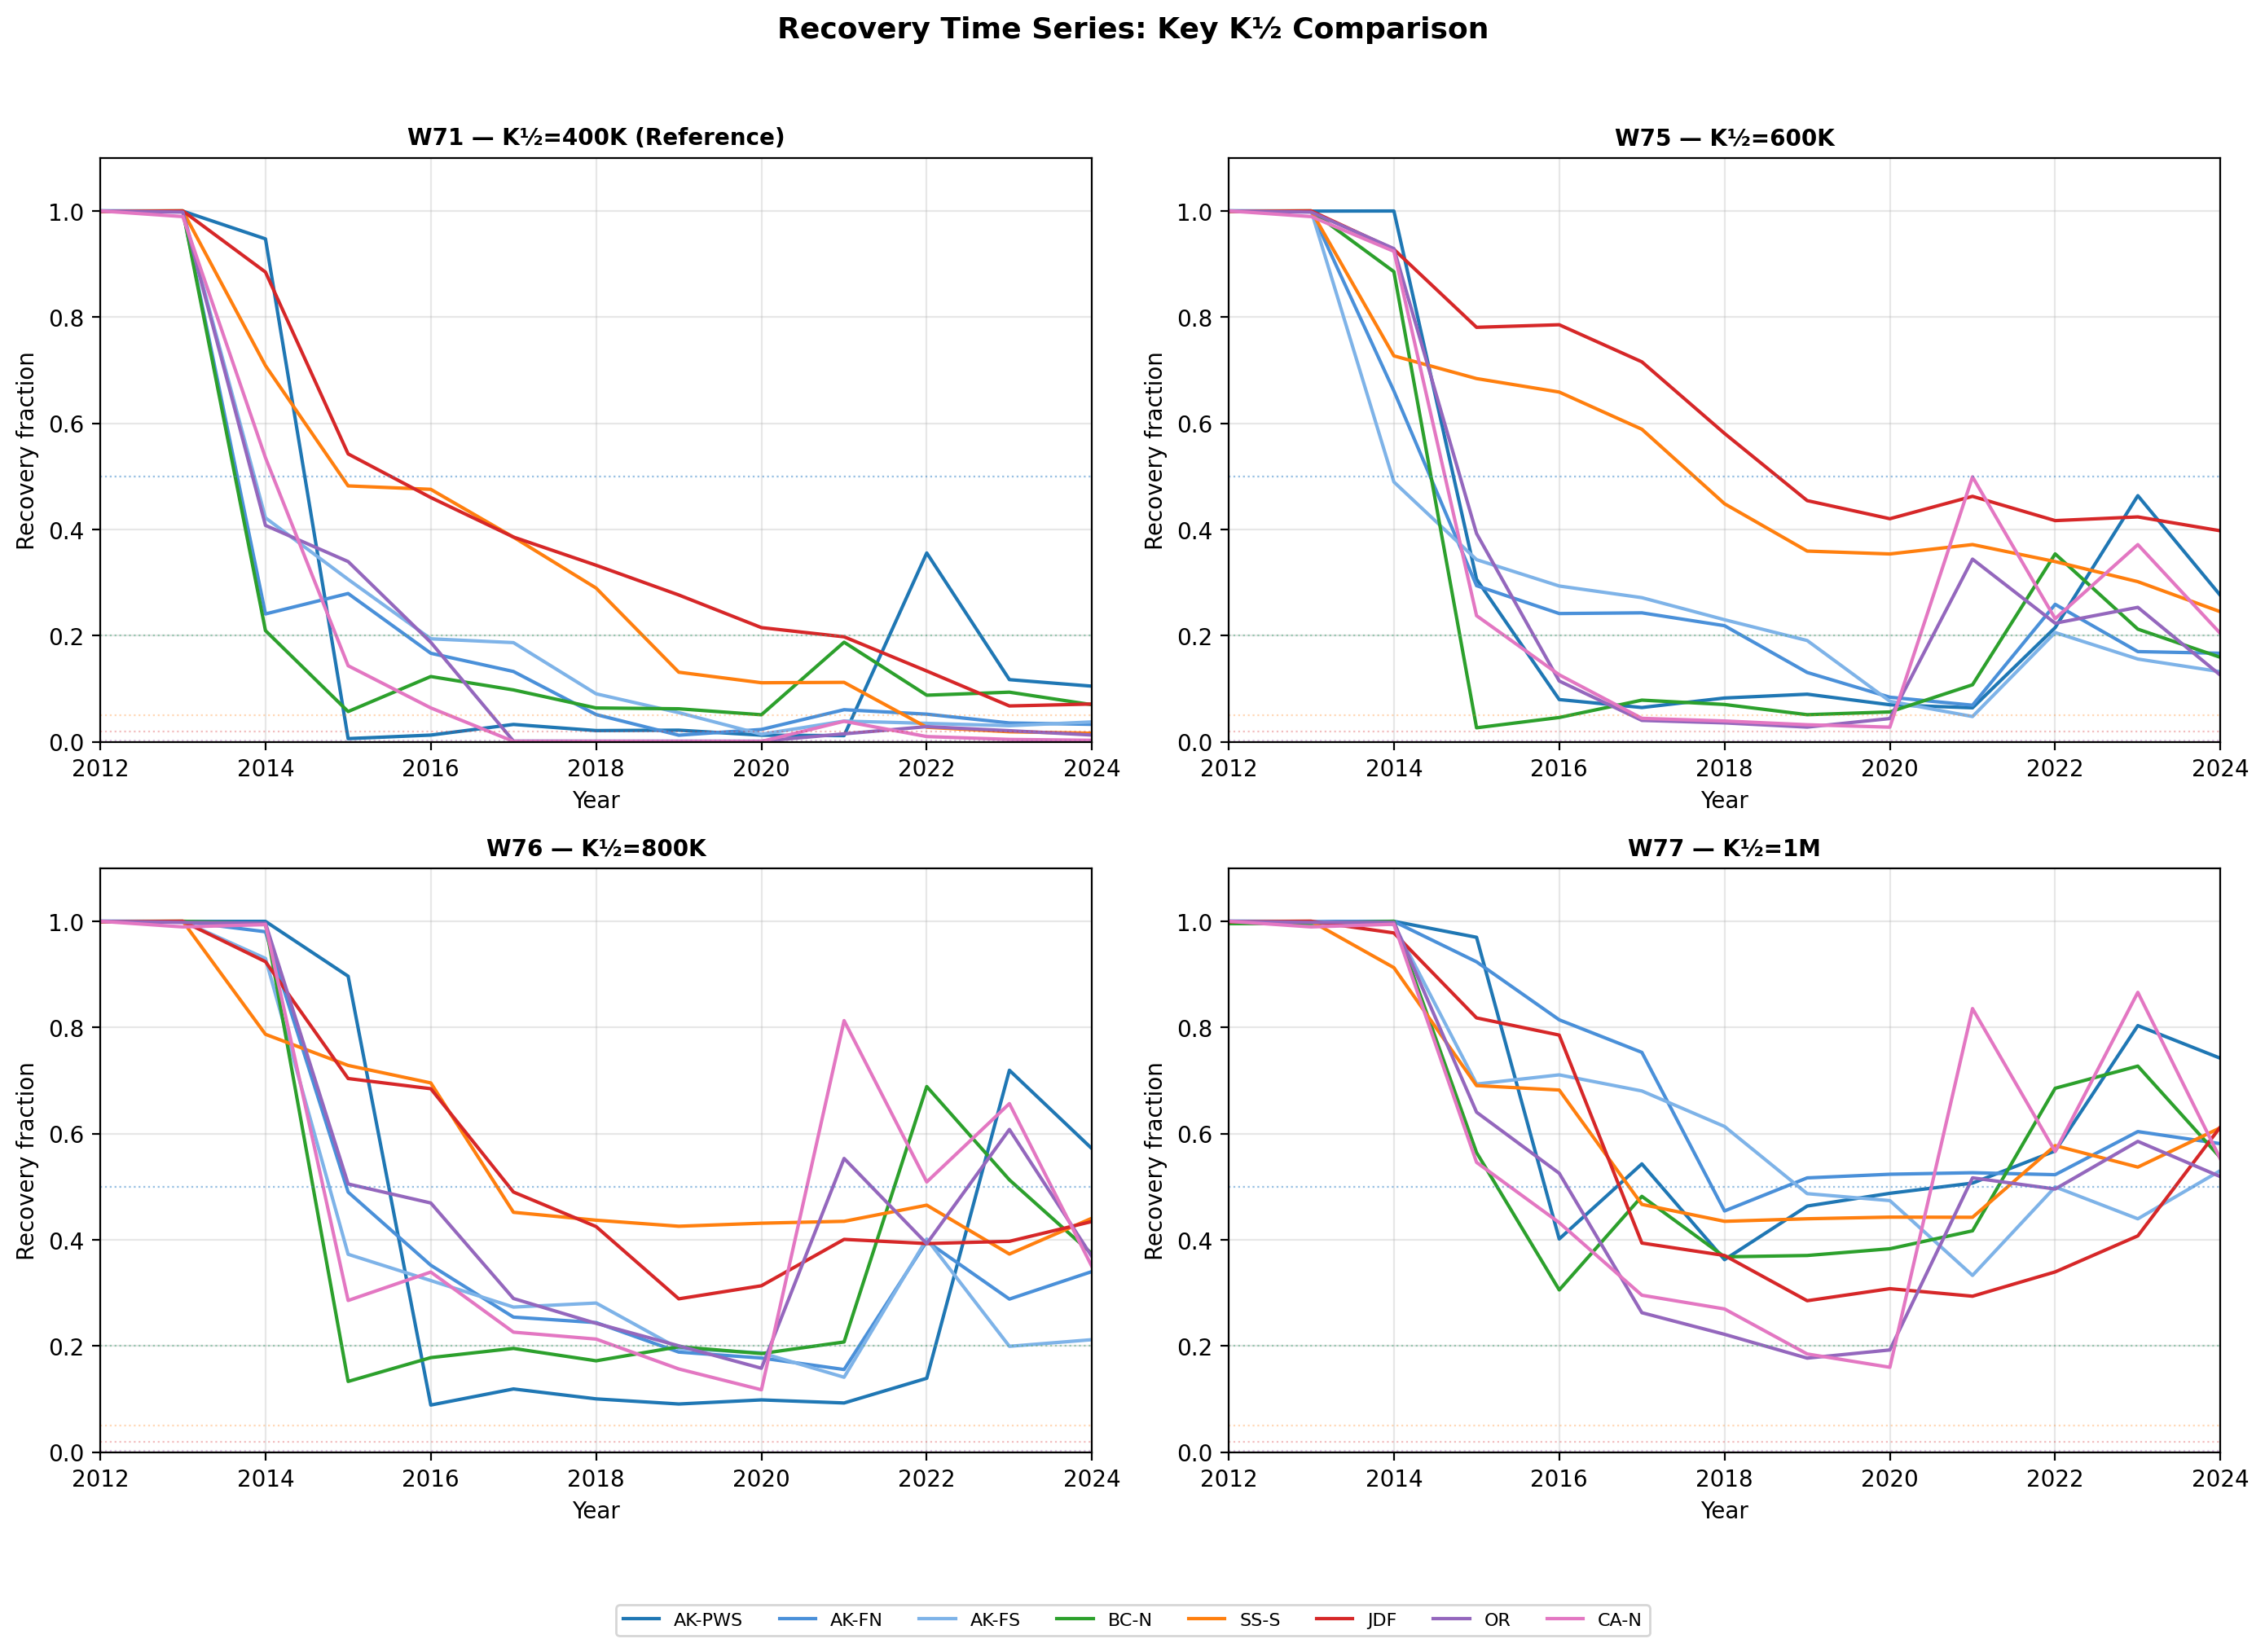
\includegraphics[width=\textwidth]{figures/fig1_key_runs_recovery.png}
\caption{Recovery time series for four key runs spanning the $K_{1/2}$ range. W71 (reference) shows suppressed but gradient-preserving recovery. As $K_{1/2}$ increases from 600K to 1M, all regions lift together, destroying the north--south gradient.}
\label{fig:key_runs}
\end{figure}

\subsection{All Runs Grid}

\begin{figure}[H]
\centering
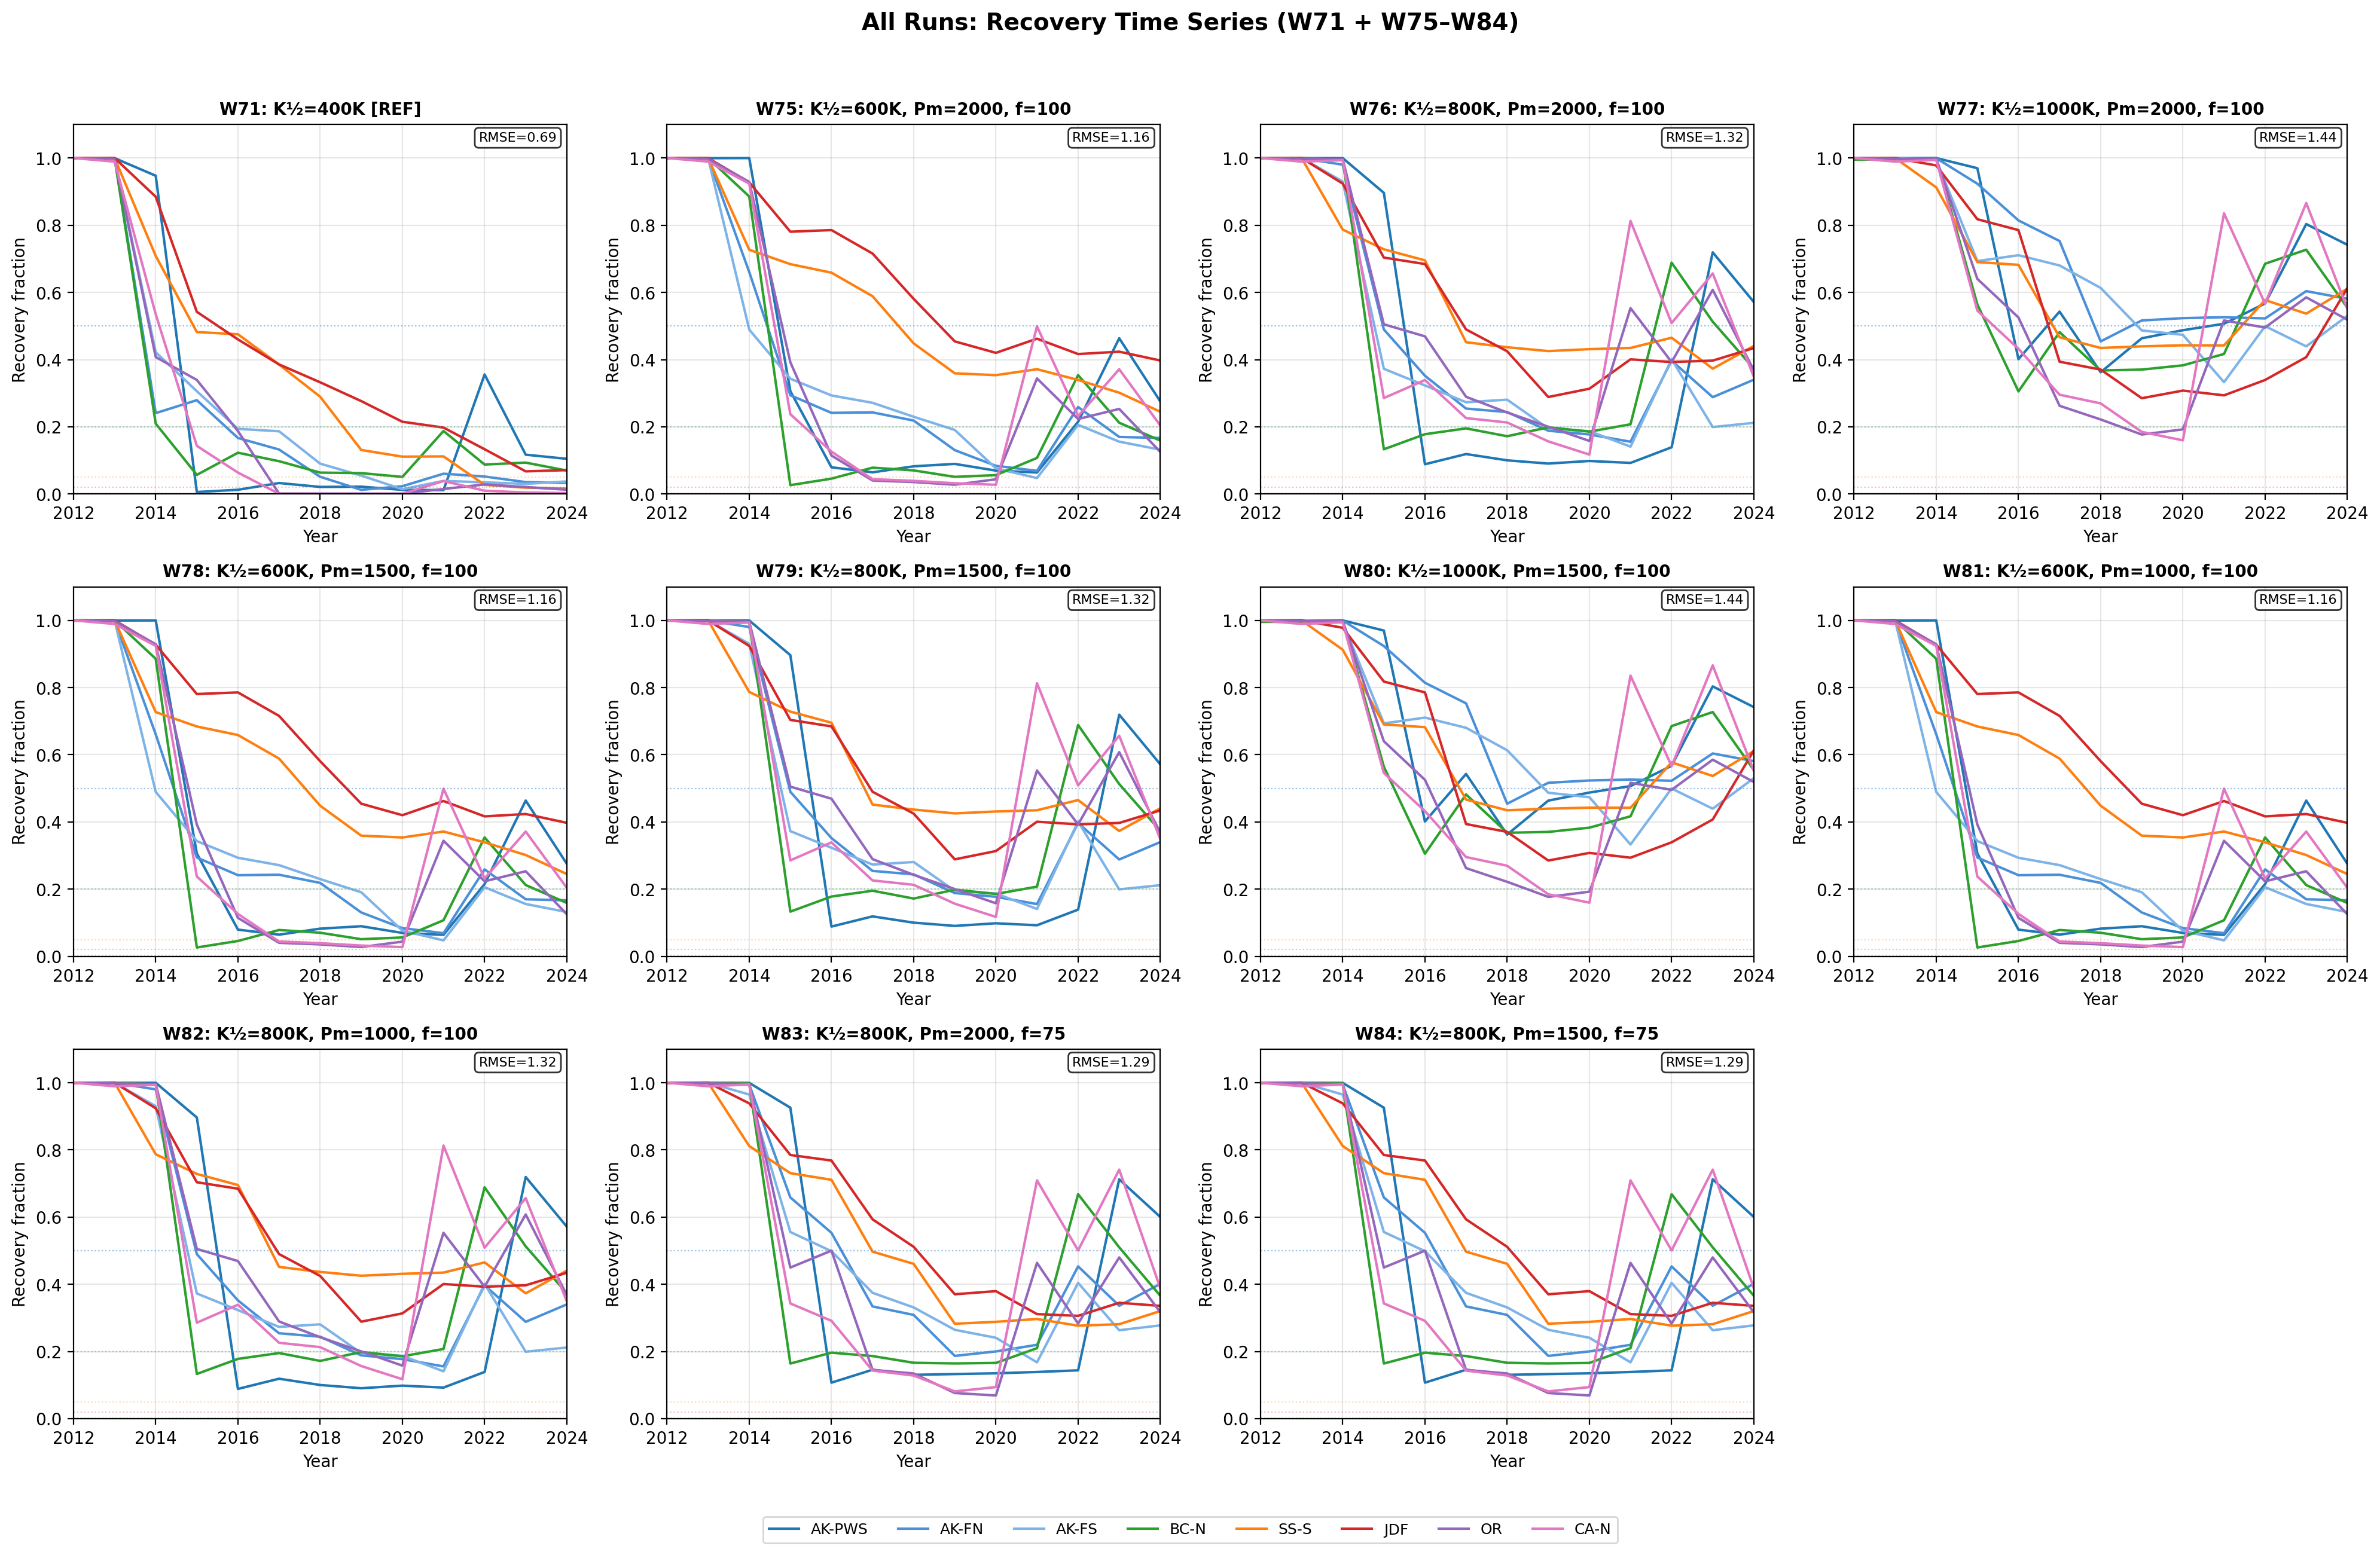
\includegraphics[width=\textwidth]{figures/fig2_all_runs_grid.png}
\caption{Recovery time series for all 11 runs (W71 reference + W75--W84). Visually identical panels within each $K_{1/2}$ group confirm $P_{\text{env,max}}$ irrelevance.}
\label{fig:all_runs}
\end{figure}

\subsection{$K_{1/2}$ Effect}

\begin{figure}[H]
\centering
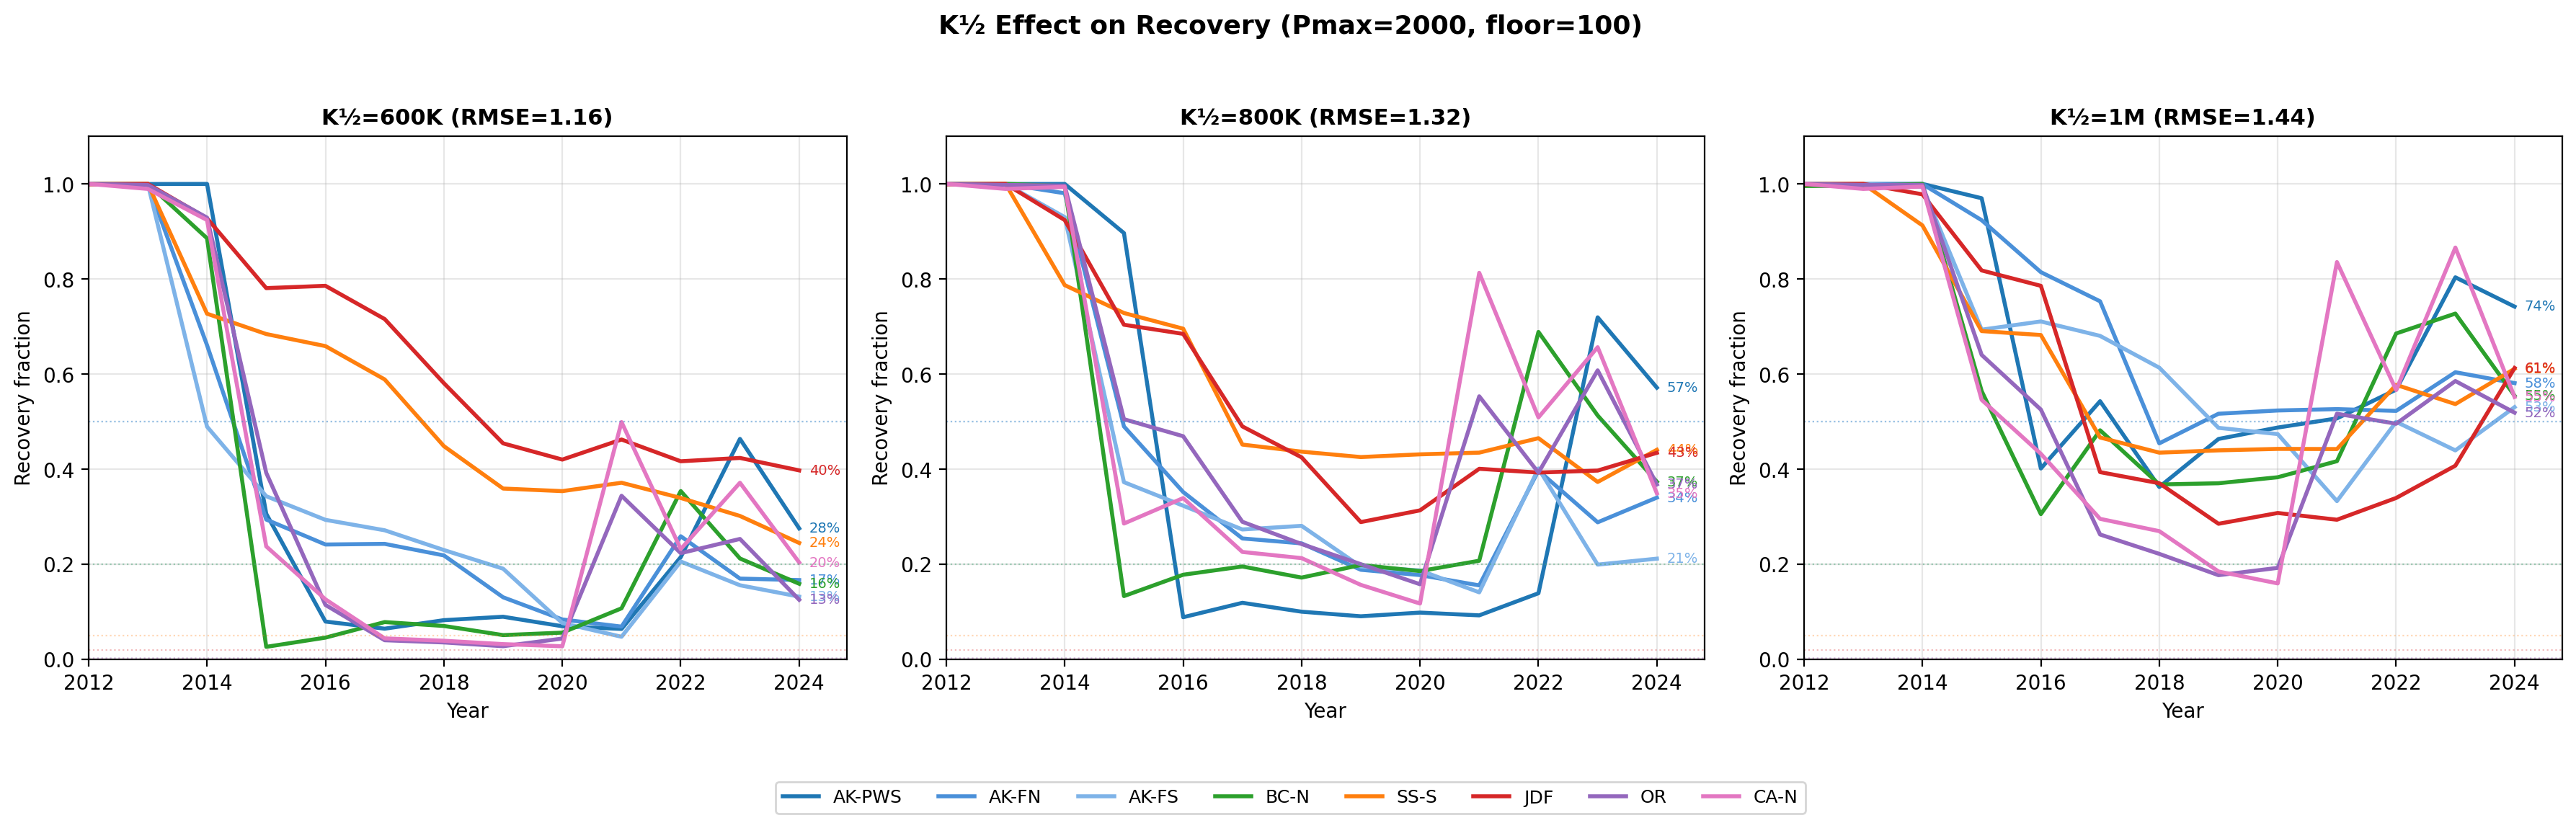
\includegraphics[width=\textwidth]{figures/fig3_khalf_effect.png}
\caption{$K_{1/2}$ effect at fixed $P_{\text{env,max}}=2000$, floor$=100$. The key observation: all recovery curves lift uniformly. At $K_{1/2}$=800K, AK-PWS$\approx$57\% matches the 50\% target, but CA-N is at 35\% instead of 0.1\%.}
\label{fig:khalf_effect}
\end{figure}

\subsection{Recovery Comparison: W71 vs W76 vs Targets}

\begin{figure}[H]
\centering
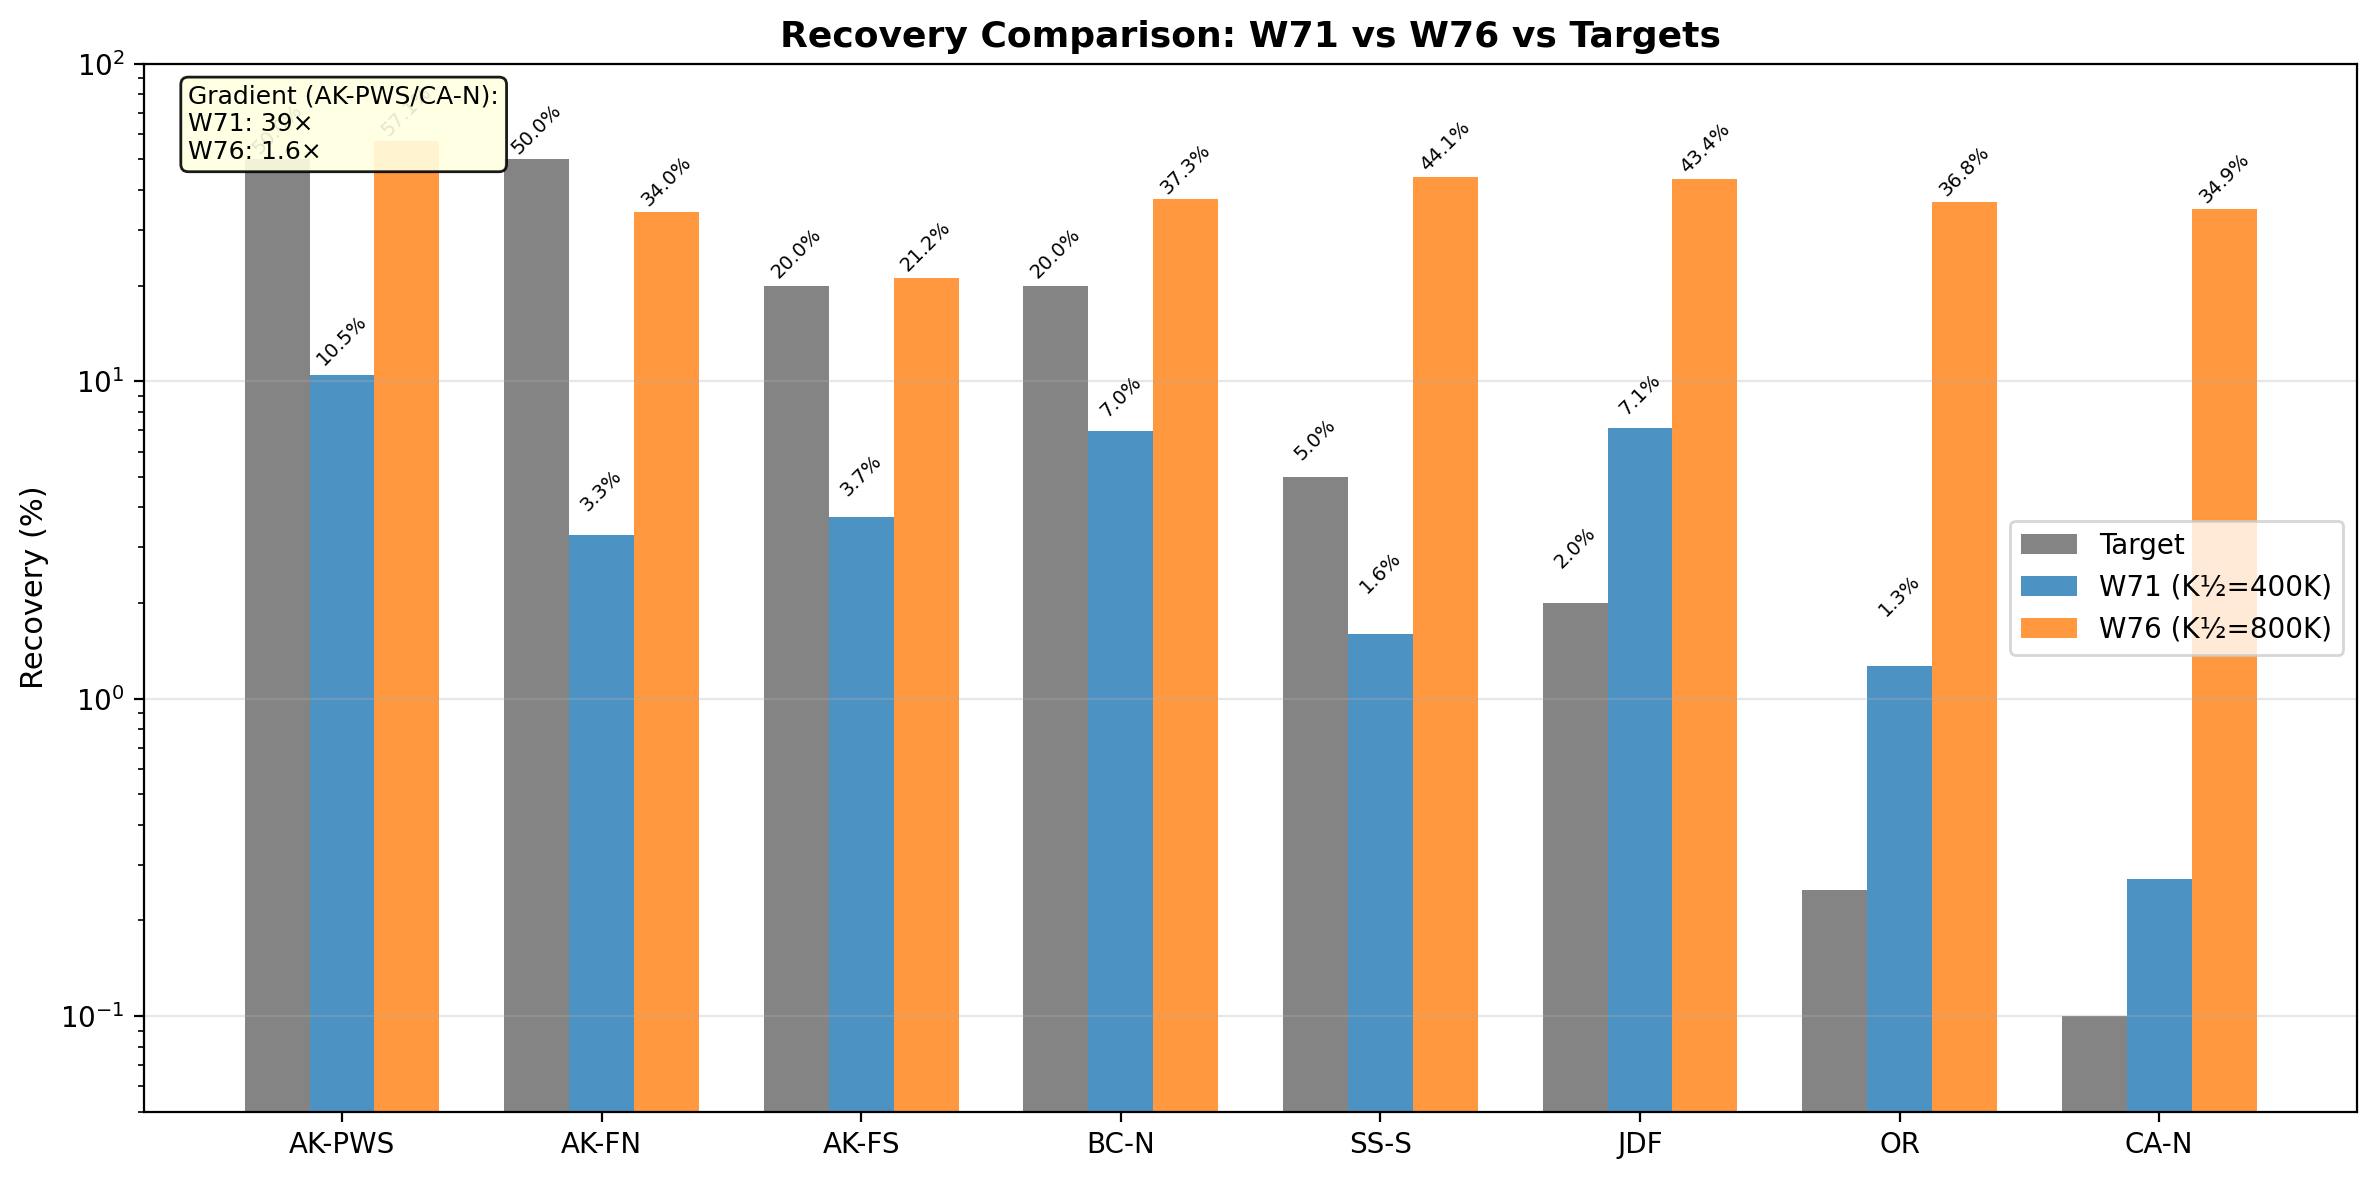
\includegraphics[width=\textwidth]{figures/fig4_recovery_comparison.png}
\caption{Bar chart comparing targets, W71, and W76 on a log scale. W71 is uniformly too low but preserves gradient. W76 nails AK-PWS and AK-FS but overshoots southern regions by 100--350$\times$.}
\label{fig:bar_comparison}
\end{figure}

\subsection{$P_{\text{env,max}}$ Independence Proof}

\begin{figure}[H]
\centering
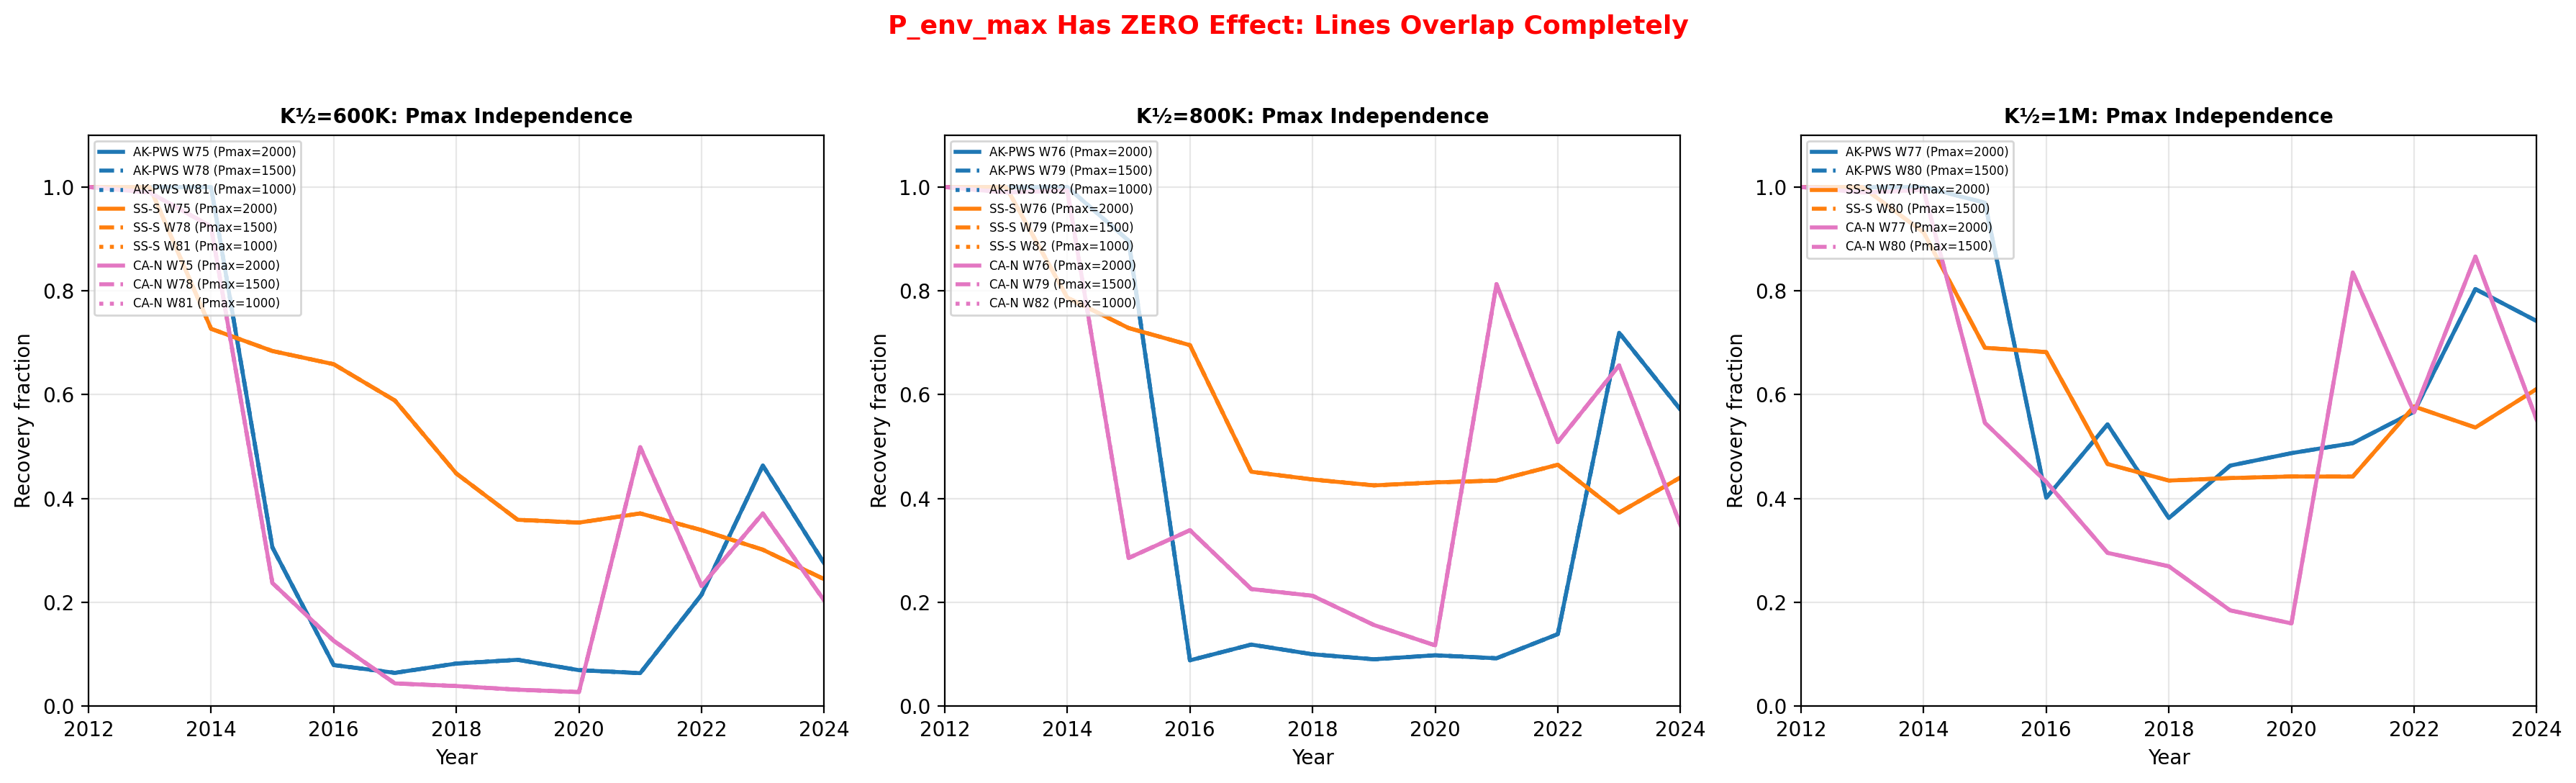
\includegraphics[width=\textwidth]{figures/fig5_pmax_independence.png}
\caption{Overlaying runs with different $P_{\text{env,max}}$ values at the same $K_{1/2}$. Lines overlap \emph{perfectly}, proving $P_{\text{env,max}}$ has zero effect when dynamic $P_{\text{env}}$ is active. Solid=$P_{\text{max}}$=2000, dashed=1500, dotted=1000.}
\label{fig:pmax_proof}
\end{figure}

\subsection{RMSE Comparison}

\begin{figure}[H]
\centering
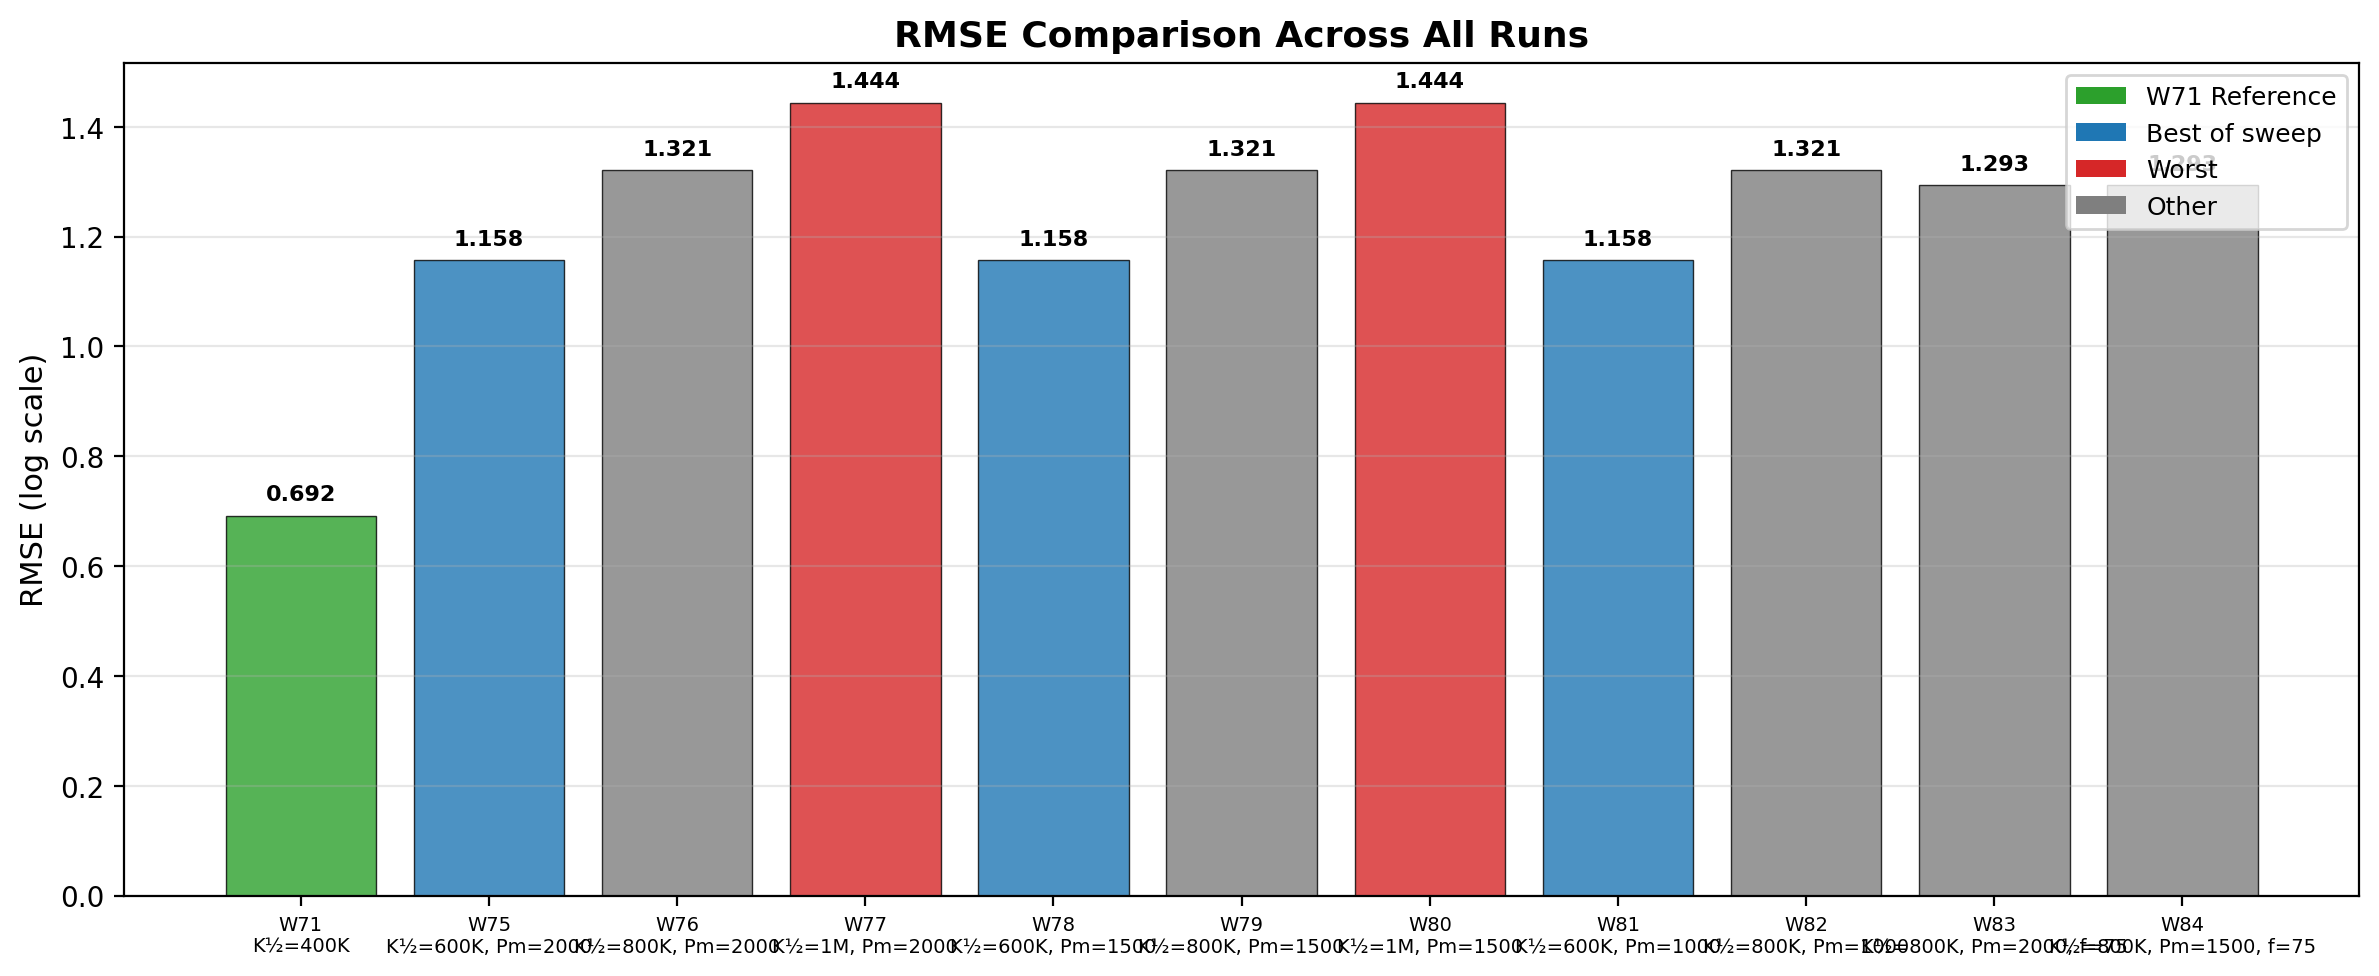
\includegraphics[width=\textwidth]{figures/fig6_rmse_comparison.png}
\caption{RMSE across all runs. W71 (green) remains best despite all values being too low. Higher $K_{1/2}$ worsens RMSE because southern overshoot grows faster than northern improvement.}
\label{fig:rmse}
\end{figure}

\subsection{Disease Dynamics (W76)}

\begin{figure}[H]
\centering
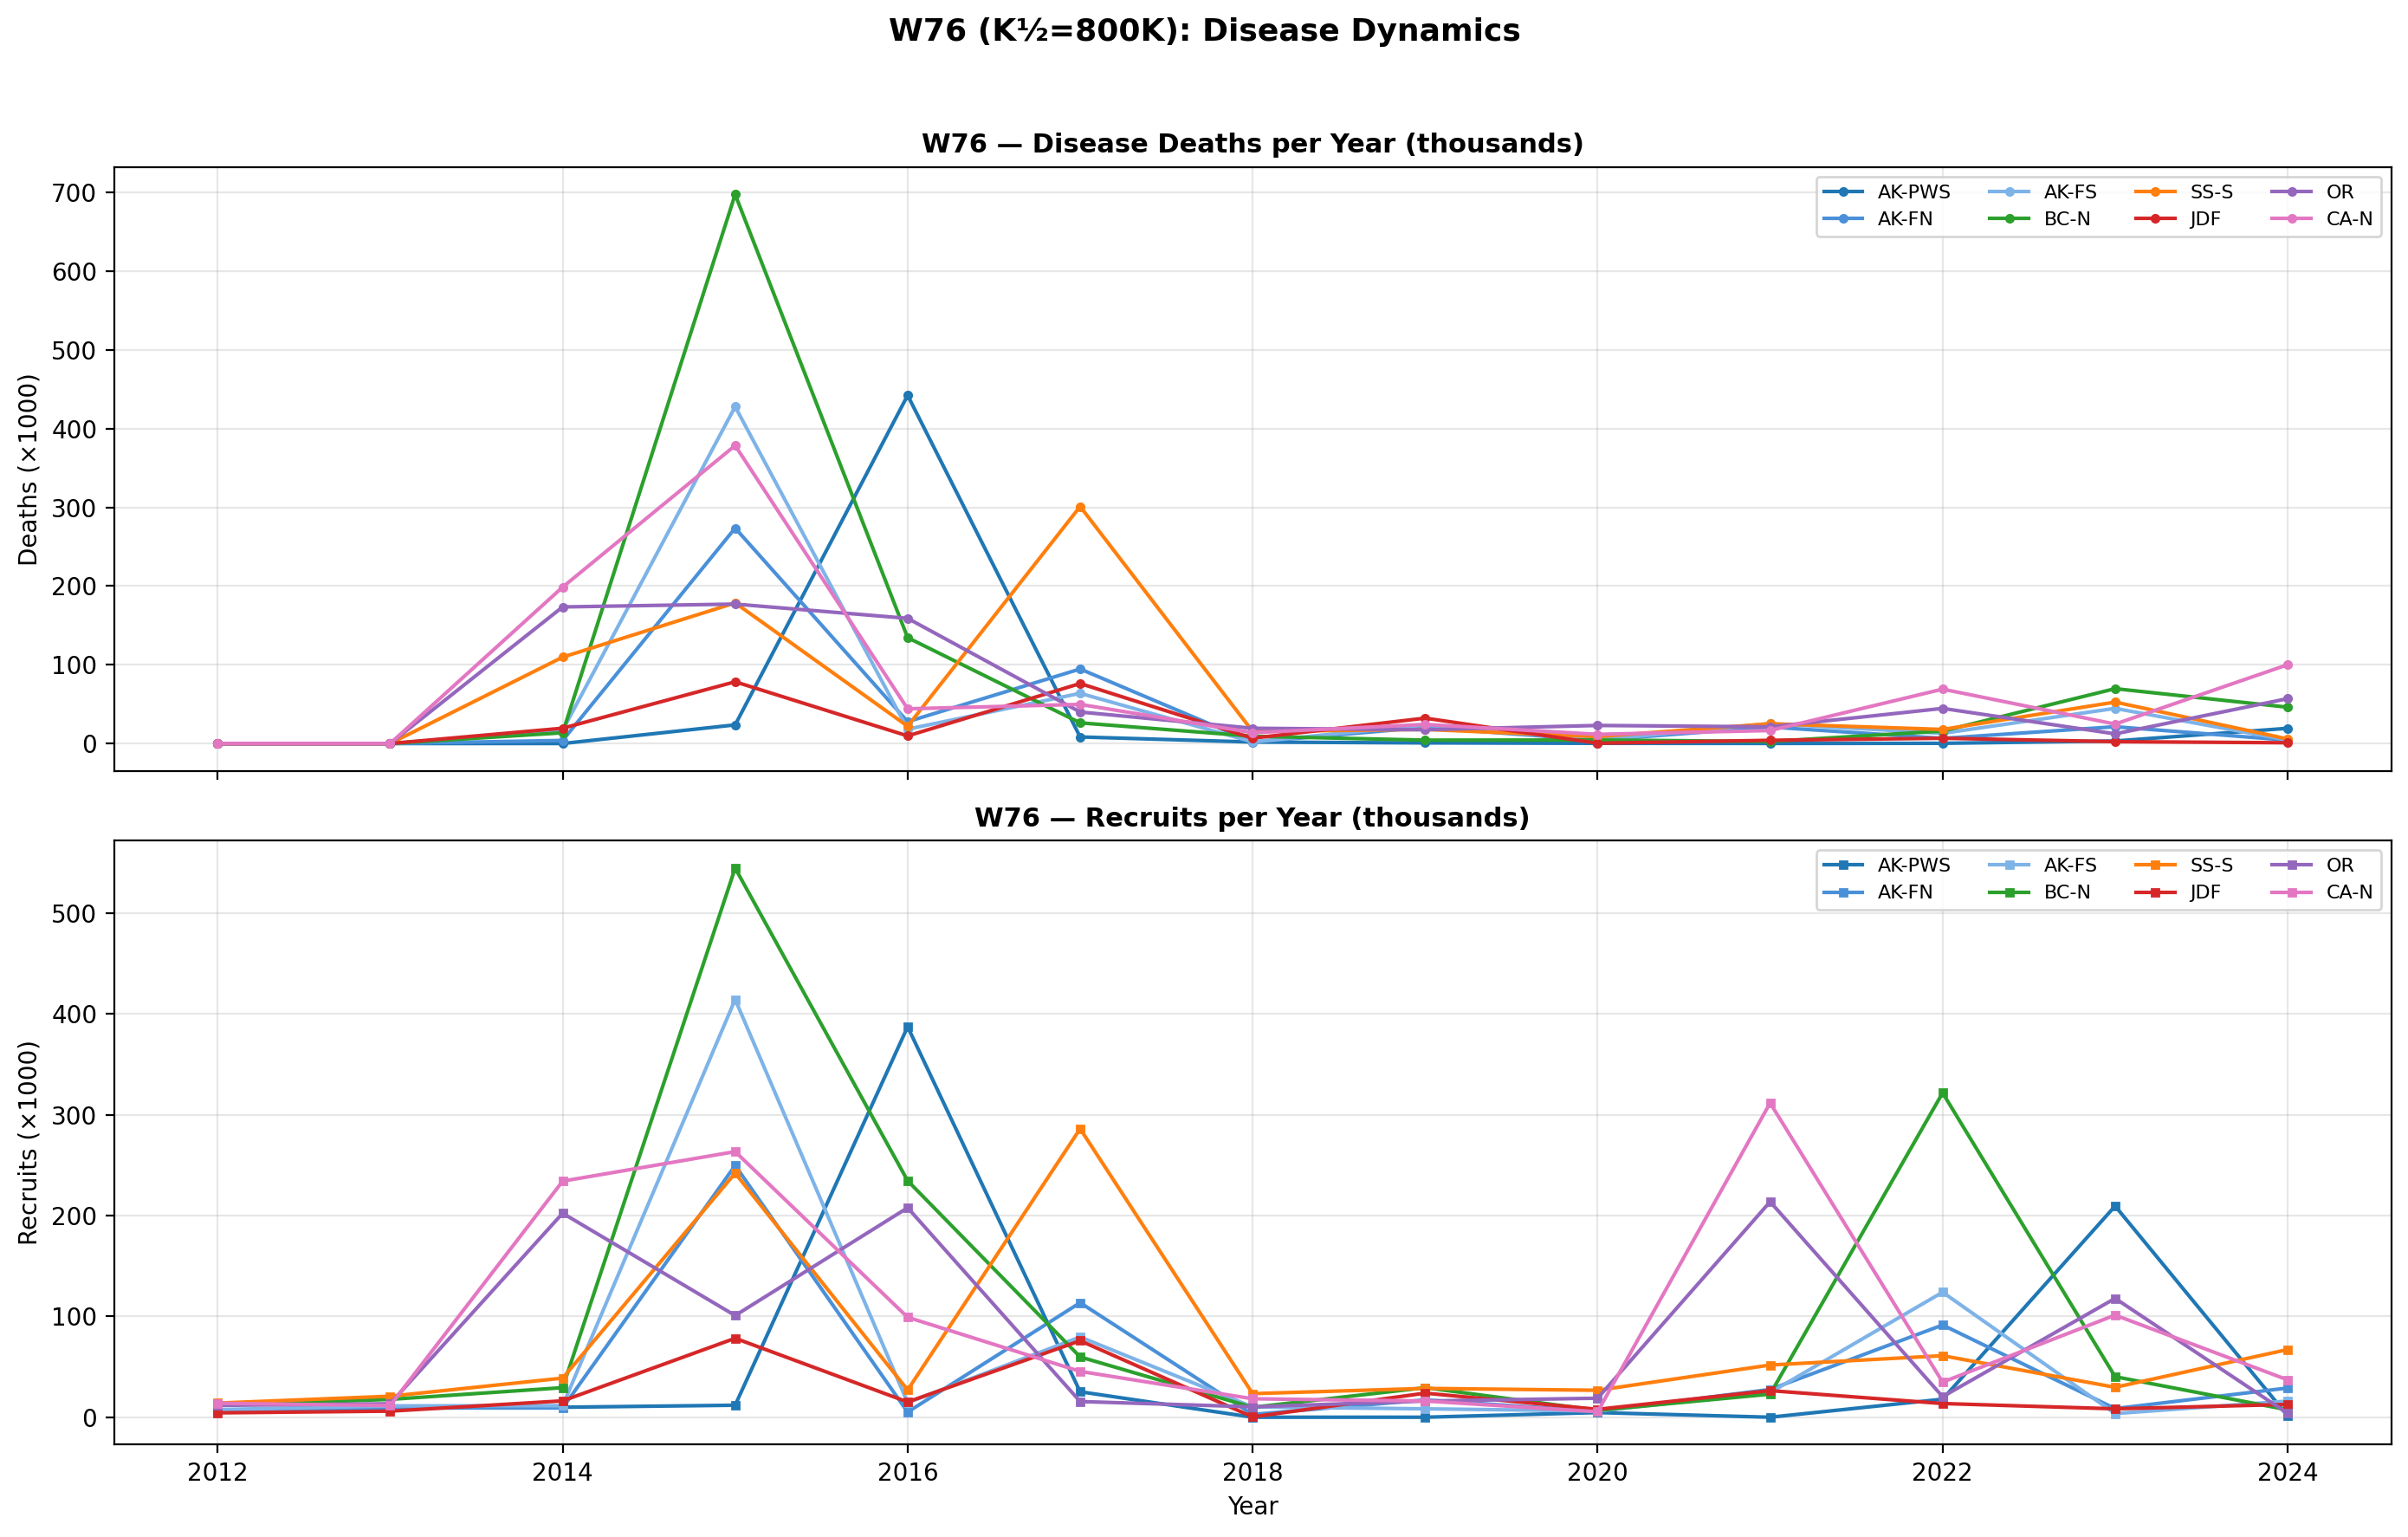
\includegraphics[width=\textwidth]{figures/fig7_disease_dynamics.png}
\caption{Disease deaths and recruitment dynamics for W76 ($K_{1/2}$=800K). Even at this higher $K_{1/2}$, disease pressure is insufficient to suppress southern populations, which rapidly recruit back to near pre-crash levels.}
\label{fig:disease}
\end{figure}

\subsection{Full Region Comparison}

\begin{figure}[H]
\centering
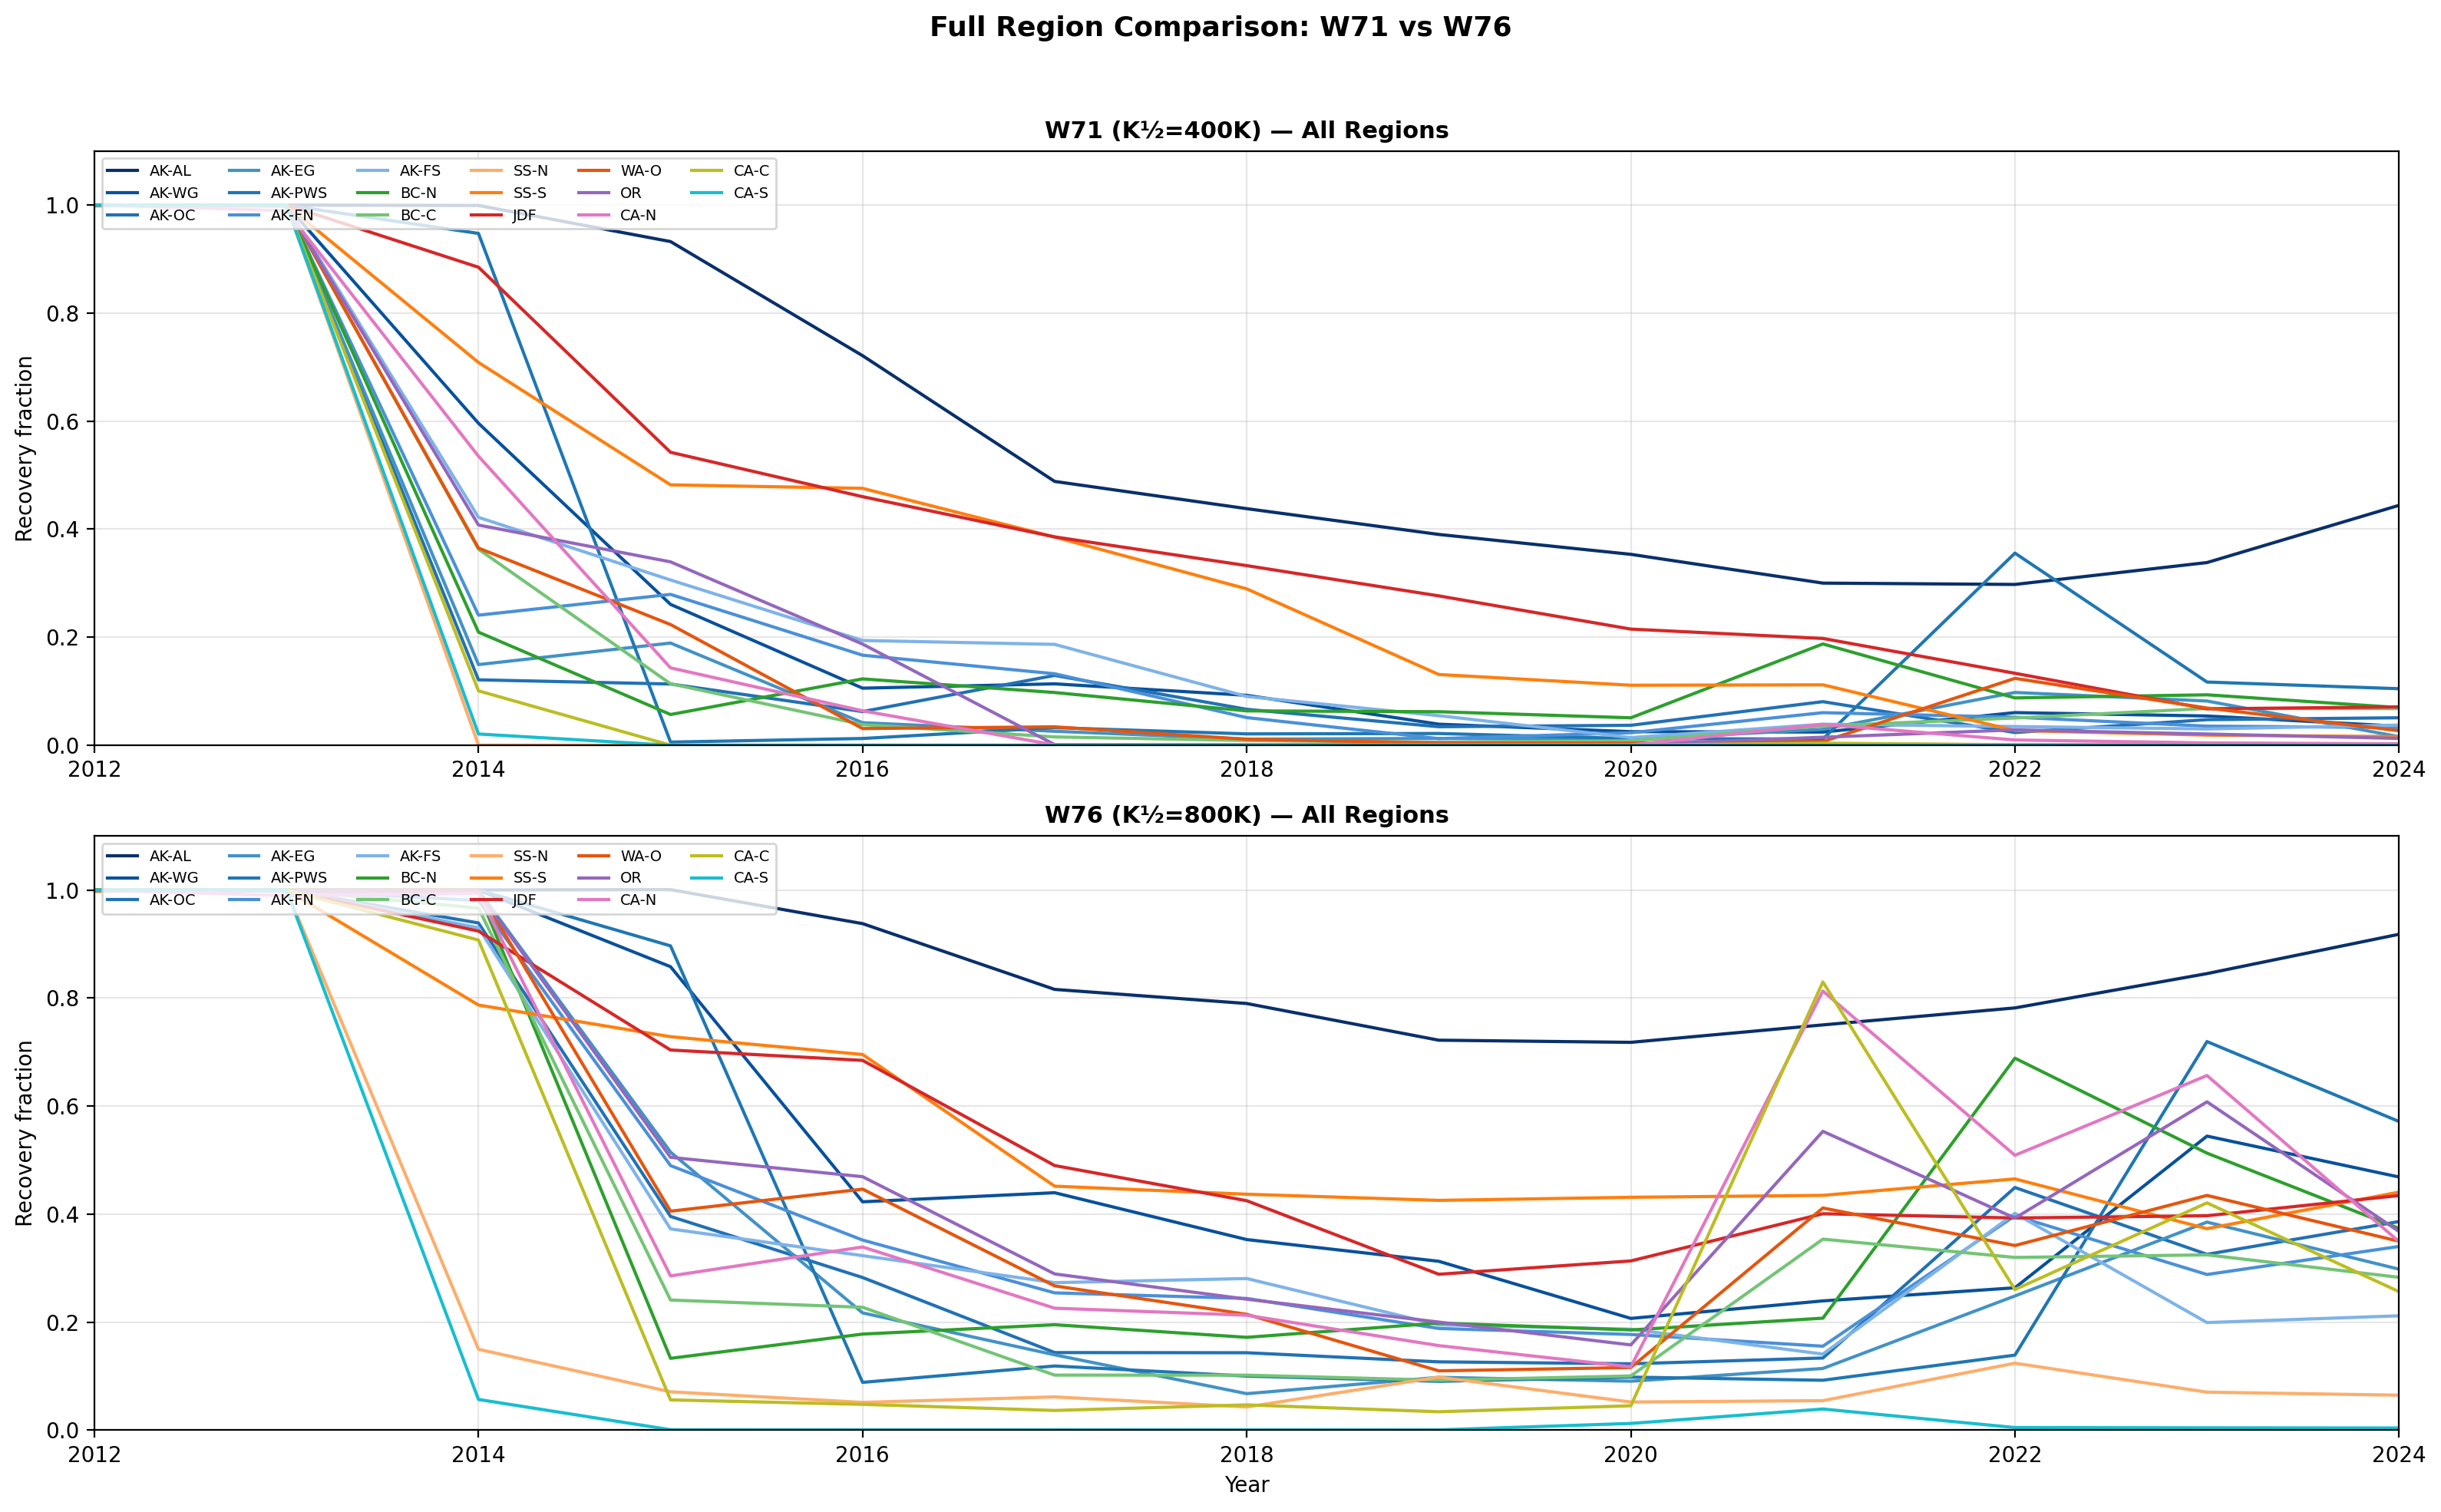
\includegraphics[width=\textwidth]{figures/fig8_full_region_comparison.png}
\caption{All modeled regions for W71 (top) and W76 (bottom). W71 shows clear north--south stratification. W76 shows near-uniform recovery across all latitudes---the gradient has effectively disappeared.}
\label{fig:full_regions}
\end{figure}


% ═══════════════════════════════════════════════════════════════
\section{Key Findings}
% ═══════════════════════════════════════════════════════════════

\subsection{Finding 1: $P_{\text{env,max}}$ Is Completely Irrelevant}

The most striking result is that $P_{\text{env,max}}$ has \textbf{exactly zero} effect on model outcomes. This is not a subtle difference---the results are identical to every decimal place:

\begin{itemize}[nosep]
    \item W75 (Pm=2000) $\equiv$ W78 (Pm=1500) $\equiv$ W81 (Pm=1000) at $K_{1/2}$=600K
    \item W76 (Pm=2000) $\equiv$ W79 (Pm=1500) $\equiv$ W82 (Pm=1000) at $K_{1/2}$=800K
    \item W77 (Pm=2000) $\equiv$ W80 (Pm=1500) at $K_{1/2}$=1M
    \item W83 (Pm=2000) $\equiv$ W84 (Pm=1500) at $K_{1/2}$=800K, floor=75
\end{itemize}

\textbf{Interpretation:} When dynamic $P_{\text{env}}$ is active, the pathogen pressure at each node never reaches the static cap. The dynamic equation ($P_{\text{env}} = P_{\text{env,floor}} + \alpha \cdot N / (N + K_{1/2})$) produces values well below even the lowest tested $P_{\text{max}}$ of 1000. This parameter can be removed from future sweeps---it is a dead parameter.

\subsection{Finding 2: $K_{1/2}$ Is a Uniform Lifter}

$K_{1/2}$ controls the ``half-saturation'' population for dynamic disease pressure. At low $K_{1/2}$ (400K, W71), disease pressure is high even at small populations, suppressing recovery everywhere. At high $K_{1/2}$ (800K--1M), disease pressure remains low until populations are very large, allowing nearly complete recovery everywhere.

The critical insight: $K_{1/2}$ affects all regions \textbf{equally}. The gradient ratio (AK-PWS / CA-N) collapses as $K_{1/2}$ increases:

\begin{center}
\begin{tabular}{lcc}
\toprule
Run & AK-PWS/CA-N ratio & Gradient quality \\
\midrule
W71 ($K_{1/2}$=400K) & 35$\times$ & Strong \\
W75 ($K_{1/2}$=600K) & 1.3$\times$ & Collapsed \\
W76 ($K_{1/2}$=800K) & 1.6$\times$ & Collapsed \\
W77 ($K_{1/2}$=1M) & 1.3$\times$ & Collapsed \\
\bottomrule
\end{tabular}
\end{center}

\subsection{Finding 3: Floor Effect Is Marginal}

Reducing $P_{\text{env,floor}}$ from 100 to 75 (W83 vs W76) produced only small changes:
\begin{itemize}[nosep]
    \item AK-PWS: 57.1\% $\to$ 60.0\% (+2.9 pp)
    \item SS-S: 44.1\% $\to$ 32.0\% ($-$12.1 pp)
    \item CA-N: 34.9\% $\to$ 38.8\% (+3.9 pp)
    \item RMSE: 1.321 $\to$ 1.293 (marginal improvement)
\end{itemize}

The floor is meant to maintain minimum disease pressure even in recovered populations, but at 75--100 it is too small to meaningfully suppress recovery. Much higher floor values (1000+) or a latitude-dependent mechanism may be needed.

\subsection{Finding 4: The Fundamental Dilemma}

The sweep reveals a fundamental structural limitation:

\begin{quote}
\textit{No single value of $K_{1/2}$ can produce both correct Alaskan recovery (50\%) and correct southern suppression (0.1--5\%). The dynamic $P_{\text{env}}$ equation with uniform parameters cannot generate a 500$\times$ gradient in recovery across regions.}
\end{quote}

This is because the dynamic $P_{\text{env}}$ responds to \textit{local} population, not latitude. Healthy populations in the south generate the same disease feedback as healthy populations in Alaska, leading to uniform recovery rates.


% ═══════════════════════════════════════════════════════════════
\section{Implications for Next Round}
% ═══════════════════════════════════════════════════════════════

The W75--W84 sweep definitively shows that the current dynamic $P_{\text{env}}$ mechanism cannot produce the required latitudinal gradient with uniform parameters. Several approaches could resolve this:

\subsection{Option A: Latitude-Dependent $K_{1/2}$}
Make $K_{1/2}$ vary by region: high in Alaska (allowing recovery) and low in the south (maintaining disease suppression). This directly addresses the gradient collapse. For example:
\begin{itemize}[nosep]
    \item Alaska: $K_{1/2}$ = 800K (proven correct for 50\% recovery)
    \item Pacific NW: $K_{1/2}$ = 200K--400K
    \item Southern: $K_{1/2}$ = 50K--100K
\end{itemize}

\subsection{Option B: Stronger Floor Mechanism}
Increase $P_{\text{env,floor}}$ dramatically in southern regions (e.g., floor=5000+ for CA/OR vs floor=100 for AK). This would create persistent disease pressure in the south regardless of population dynamics.

\subsection{Option C: Temperature-Dependent Disease Pressure}
Link disease pressure to water temperature. Southern regions have warmer water year-round, maintaining higher disease pressure. This is biologically motivated---SSWD is more virulent in warmer water.

\subsection{Option D: External Reservoir}
Add a latitude-dependent environmental disease reservoir that persists regardless of population dynamics. Southern waters maintain higher baseline pathogen levels due to warmer temperatures and higher biodiversity.

\subsection{Recommended Next Steps}
\begin{enumerate}[nosep]
    \item \textbf{Drop $P_{\text{env,max}}$ from all future sweeps}---it is a confirmed dead parameter.
    \item \textbf{Test latitude-dependent $K_{1/2}$} as the most direct fix.
    \item Consider whether $K_{1/2}$=800K is the correct AK value (57\% vs 50\% target is close).
    \item Explore temperature-mediated disease for biological realism.
\end{enumerate}


% ═══════════════════════════════════════════════════════════════
\section*{Appendix: Effective Unique Runs}
% ═══════════════════════════════════════════════════════════════

Due to $P_{\text{env,max}}$ irrelevance, the 10 W75--W84 runs reduce to only \textbf{4 distinct configurations}:

\begin{center}
\begin{tabular}{lll}
\toprule
\textbf{Configuration} & \textbf{Equivalent Runs} & \textbf{RMSE} \\
\midrule
$K_{1/2}$=600K, floor=100 & W75 = W78 = W81 & 1.158 \\
$K_{1/2}$=800K, floor=100 & W76 = W79 = W82 & 1.321 \\
$K_{1/2}$=1M, floor=100 & W77 = W80 & 1.444 \\
$K_{1/2}$=800K, floor=75 & W83 = W84 & 1.293 \\
\bottomrule
\end{tabular}
\end{center}

\end{document}
